% Template for ICIP-2014 paper; to be used with:
%          spconf.sty  - ICASSP/ICIP LaTeX style file, and
%          IEEEbib.bst - IEEE bibliography style file.
% --------------------------------------------------------------------------
\documentclass{article}
\usepackage{spconf,amsmath,graphicx}

% Example definitions.
% --------------------
\def\x{{\mathbf x}}
\def\L{{\cal L}}

% Title.
% ------
\title{Vertex Extraction for Convex and Concave Polygons}
% TODO 进行拼写检查
%
% Single address.
% ---------------
\name{Zhou Xiong}
\address{Harbin Institute of Technology\\Computer Science and Engneering\\Harbin, China}

%
% For example:
% ------------
%\address{School\\
%       Department\\
%       Address}
%
% Two addresses (uncomment and modify for two-address case).
% ----------------------------------------------------------
%\twoauthors
%  {A. Author-one, B. Author-two\sthanks{Thanks to XYZ agency for funding.}}
%       {School A-B\\
%       Department A-B\\
%       Address A-B}
%  {C. Author-three, D. Author-four\sthanks{The fourth author performed the work
%       while at ...}}
%       {School C-D\\
%       Department C-D\\
%       Address C-D}
%
\begin{document}
%\ninept
%
\maketitle
%
\begin{abstract}

Locating the vertices of a polygonal digital contour is an important but seldomly addressed problem.
We propose two fast and robust methods for vertex detection in convex and non-convex polygons.
The first method is dedecated to convex polygons. We first map each point to the unit circle, then apply
k-means to assign points the corresponding lines, vertices are computed as the intersection of adjacent lines.
The mapping in the method can preserve the topological order of points, which is a key contribution of our method.
The second method does not require the polygon to be convex. We use the RANSAC approach to fit the polygon. A polygon
is modelded as consecutive lines, we iterate several times and choose the model with highest inliner rate. Expriemnts
on natural and synthetical images are given to show the validity of our approach.

\end{abstract}
%
\begin{keywords}
  Vertex detection, Convex Hull, K-means, RANSAC
\end{keywords}
%
\section{Introduction}
\label{sec:intro}
The work on the detection of dominant points started from the research of Attneave who proposed that the local maximum
curvature points on a curve have a rich information content and are sufficient to characterize this curve have a rich
rich infomation content and are sufficient to characterize this curve. A method for detection of
dominant points can lead to a good representation of a planar shape at different resolutions.

In addition, a representation of a planar shape based on dominant points has some advantages.
Firstly, it enables a high data reduction.
Secondly, this representation concentrates on principal features of the shape, so it is
efficient for shape matching, feature extraction or decomposition of curve into meanningful parts.
Therefore, these points have a critical role in curve approximation, shape matching and image matching.
They also lead to some applications in other domains of machine vision such as vector data compression.

Starting from Attneave's work, there are many existing methods for dominant points detection.
Concerning this problem, several problems in this topic have been identified: evaluation, number of
parameters, selection of starting point, multi-scale, working with noisy curves, \dots.

In general, we can classify these methods into two groups.
The first one contains direct methods that determine dominant points such as high curvature
value points by using curvature-based significant measures, or using alternative significant
measures such as k-cosine, region of support (ROS). Rosenfield and Johnston used cosine of the
angle between the archs of length k on each side of a point (termed k-cosine) as curvature-based
significant measure.
The indirect methods are often based on polygonal approxiamation of the curve,
the dominant points are deduced after doing this step.
In these methods, the dominant points are detected as the vertex of approximated polygons.
In addition, we can divide polygonal approximation methods into three principal approaches:
sequential approach, split and merge approch, heuristic search one.
For sequential approach, Ray and Ray determined the longest possible line segement
with minimum error. Kolesnikov proposed a sub-optimal algorithm for polygon
approximation of closed curves based on the corresponding optimal dynamic programming
algorithm for open curves.
Aoyama used a linear scan to evaluate error condtions, if the conditions are not satisfied,
a new segment search is started. The problem of this method is that sometimes the nodes
do not correspond to the corners because a new vector is defined only when the condtions
are violated.
For split-and-merge methods, lines are fitted to an intial segmentation of the boundary
and then the least square error is computed. These methods then iteratively split
a line if the error is too large and merge two points if the error is too small.
Heuristic approach is used to reduce the complexity of an optimal algorithm for approximating
polygon. Genetic algorithm, tabu search, ant colony search, fuzzy ressning are some
popular techniques approach is simple and fast, but the quality of its result depends on the
starting point.
Masood has proposed an efficient method taht does not belong to any of the above groups.
It is based on break point extraction. A break point is a point of which the chain code
is different from that of the previous point. Break points are taken as initial set of
dominat points. Each break point are taken as initial set of dominant points.

\subsection{Hough Transform}
\label{sub:Hough Transform}

\subsection{Previous Methods}
\label{sub:Previous Methods}

\subsection{Critical Point}
\label{sub:Critical Point}

\subsection{Polygonal Approximation}
\lable{sub:polygon}

\subsection{Computational Geometry}
\label{sub:Computational Geometry}

\subsection{My Method}
\label{sub:My Method}

We adopt ideas from data clustering and machine vision

\section{MAJOR HEADINGS}
\label{sec:majhead}

Major headings, for example, ``1. Introduction'', should appear in all capital
letters, bold face if possible, centered in the column, with one blank line
before, and one blank line after. Use a period (``.'') after the heading number,
not a colon.

\subsection{Subheadings}
\label{ssec:subhead}

Subheadings should appear in lower case (initial word capitalized) in
boldface.  They should start at the left margin on a separate line.

\subsubsection{Sub-subheadings}
\label{sssec:subsubhead}

Sub-subheadings, as in this paragraph, are discouraged. However, if you
must use them, they should appear in lower case (initial word
capitalized) and start at the left margin on a separate line, with paragraph
text beginning on the following line.  They should be in italics.

\section{PAPER FORMAT}
\label{sec:print}

Format you paper for US letter, $8.5 \times 11$-inch paper.
A4 paper is also acceptable, but please leave the extra 0.5 inch (12 mm)
empty at the BOTTOM of the page and follow the top and left margins as
specified.  If the last page of your paper is only partially filled, arrange
the columns so that they are evenly balanced if possible, rather than having
one long column.

In LaTeX, to start a new column (but not a new page) and help balance the
last-page column lengths, you can use the command ``$\backslash$pagebreak'' as
demonstrated on this page (see the LaTeX source below).

\section{PAGE NUMBERING}
\label{sec:page}

Please do {\bf not} paginate your paper.  Page numbers, session numbers, and
conference identification will be inserted when the paper is included in the
proceedings.

\section{ILLUSTRATIONS, GRAPHS, AND PHOTOGRAPHS}
\label{sec:illust}

Illustrations must appear within the designated margins.  They may span the two
columns.  If possible, position illustrations at the top of columns, rather
than in the middle or at the bottom.  Caption and number every illustration.
All halftone illustrations must be clear black and white prints.  Colors may be
used, but they should be selected so as to be readable when printed on a
black-only printer.

Since there are many ways, often incompatible, of including images (e.g., with
experimental results) in a LaTeX document, below is an example of how to do
this \cite{Lamp86}.

\section{FOOTNOTES}
\label{sec:foot}

Use footnotes sparingly (or not at all!) and place them at the bottom of the
column on the page on which they are referenced. Use Times 9-point type,
single-spaced. To help your readers, avoid using footnotes altogether and
include necessary peripheral observations in the text (within parentheses, if
you prefer, as in this sentence).

% Below is an example of how to insert images. Delete the ``\vspace'' line,
% uncomment the preceding line ``\centerline...'' and replace ``imageX.ps''
% with a suitable PostScript file name.
% -------------------------------------------------------------------------
\begin{figure}[t]

\begin{minipage}[b]{1.0\linewidth}
  \centering
  \centerline{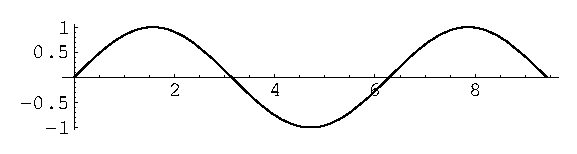
\includegraphics[width=8.5cm]{Figures/image1}}
%  \vspace{2.0cm}
  \centerline{(a) Result 1}\medskip
\end{minipage}
%
\begin{minipage}[b]{.48\linewidth}
  \centering
  \centerline{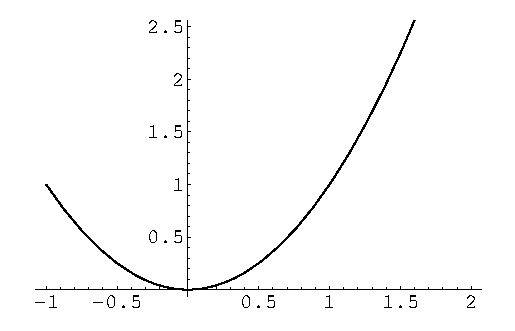
\includegraphics[width=4.0cm]{Figures/image3}}
%  \vspace{1.5cm}
  \centerline{(b) Results 3}\medskip
\end{minipage}
\hfill
\begin{minipage}[b]{0.48\linewidth}
  \centering
  \centerline{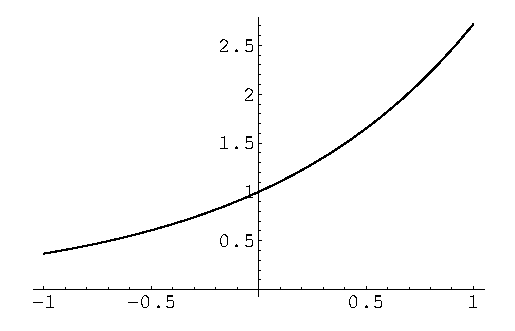
\includegraphics[width=4.0cm]{Figures/image4}}
%  \vspace{1.5cm}
  \centerline{(c) Result 4}\medskip
\end{minipage}
%
\caption{Example of placing a figure with experimental results.}
\label{fig:res}
%
\end{figure}


% To start a new column (but not a new page) and help balance the last-page
% column length use \vfill\pagebreak.
% -------------------------------------------------------------------------
%\vfill
%\pagebreak

\section{COPYRIGHT FORMS}
\label{sec:copyright}

You must include your fully completed, signed IEEE copyright release form when
form when you submit your paper. We {\bf must} have this form before your paper
can be published in the proceedings.

\section{REFERENCES}
\label{sec:ref}

List and number all bibliographical references at the end of the
paper. The references can be numbered in alphabetic order or in
order of appearance in the document. When referring to them in
the text, type the corresponding reference number in square
brackets as shown at the end of this sentence \cite{C2}. An
additional final page (the fifth page, in most cases) is
allowed, but must contain only references to the prior
literature.

% References should be produced using the bibtex program from suitable
% BiBTeX files (here: refs). The IEEEbib.bst bibliography
% style file from IEEE produces unsorted bibliography list.
% -------------------------------------------------------------------------
\bibliographystyle{IEEEbib}
\bibliography{refs}

\end{document}
